\documentclass[twocolumn]{article}
% \usepackage{mathptmx}  % Postscript fonts for math mode
\usepackage{amsmath}
\usepackage{amsthm}
\usepackage{amsfonts}
\usepackage{amssymb}
\usepackage{graphicx}
\usepackage{url}
\usepackage{color}    % Used to highlight comments
\usepackage{cite}
\usepackage{indentfirst}
\usepackage[ruled]{algorithm2e}
\usepackage[bookmarks=false]{hyperref}

\newcommand{\psz}[1]{\textcolor{red}{\footnotesize [PSz: #1]}}
\usepackage{listings}
\usepackage{xcolor}
\lstset{
    numbers=left, 
    numberstyle= \tiny, 
    keywordstyle= \color{ blue!70},
    commentstyle= \color{red!50!green!50!blue!50}, 
    frame=shadowbox, % 阴影效果
    rulesepcolor= \color{ red!20!green!20!blue!20} ,
    escapeinside=``, % 英文分号中可写入中文
    xleftmargin=2em,xrightmargin=2em, aboveskip=1em,
    framexleftmargin=2em
}

%--------------------------------------------------------------------------------

\title{ACTGS: Access Control Tickets-Generate Service for Smart Contract}
\author{$Bowen Liu^{1}$, $Chunpeng Ge^{2}$, $Pawel Szalachowski^{2}$\\
    \small{$^{1,2}$Department of Information Systems Technology and Design}\\
    \small{$^{1,2}$Singapore University of Technology and Design, Singapore}\\
    \small{$^{1}$bowen\_liu@mymail.sutd.edu.sg, $^{2}$chunpeng\_ge, pawel@sutd.edu.sg}\\
}
\date{}

%--------------------------------------------------------------------------------

\begin{document}
\maketitle

\begin{abstract}
- Briefly motivate problem domain, why is it an imporant domain?
- What problem does the paper solve?
- What is the main contribution?
-> The abstract should convince a reader to read the paper, not
  necessary to explain anything, just provide an incentive to read
- Keep the abstract short! Should be fewer than 15 lines.
\psz{test}
\end{abstract}

\section{Introduction}
\label{sec:intro}
1) Give a general background -> give specific background -> Mention previous
research
2) Look for a niche
3) Introduce your own paper -> State your research aims


- Motivate problem, show that it's an important and difficult problem
  - Solve a very specific problem
- Paint the research landscape, explain deficiency of current state of
  the art, explain what aspect your research addresses. Explain how
  the current paper fits into the research landscape.
  What is the ultimate research goal in this area? How does the
  current paper help to get us closer towards that goal?
- Explain what the main research challenge is, why is it a difficult
  and important problem? This is very important, if the audience
  agrees that the challenge is difficult (they don't know how to solve
  it) and important, the paper is almost already accepted.
  State interesting questions that the paper addresses.
- Provide a very explicit, verifiable claim for a metric for approach
  (we propose system X with property Y, Y must be easy to measure and
   clear to see merit wrt related work)
  If one can show that we made verifiable progress on a relevant
  problem, then the paper cannot be rejected :-)
- Explain KEY CONCEPTS / INSIGHTS that the paper introduces
- Pose a list of QUESTIONS! Readers love puzzles, and ideally, the
  paper contains several questions that the reader will try to answer
  but can't, then once the answer is in the paper the reader says: great!
- List of CONTRIBUTIONS


\section{Background}
\label{sec:pre}
Background
Problem Definition
- Clear and concise problem formulation
- Present specific quality metric for evaluation
Attacker Model
Assumptions

The notation used throughout the paper is presented in \autoref{tab:notation}
\begin{table}[h!]
\begin{center}
% \renewcommand*{\arraystretch}{1.25}
    \begin{tabular}{ll}
$\{msg\}_A$ & denotes the message $msg$ digitally signed by $A$, \\
$h(.)$ & is a cryptographic hash function, \\
$\|$ & is the string concatenation, \\
$r\xleftarrow{R}S$ & denotes that $r$ is an element randomly selected from the set $S$,\\
$\{0,1\}^n$ & is a set of all $n$-bit long strings,\\
$t_x$ & is a Unix timestamp expressed in seconds. \\
\end{tabular}
\end{center}
    \caption{Notation used throughout the paper.}
    \label{tab:notation}
\end{table}
\\\textit{A. Blockchain and Smart Contracts}
- Introduce consensus, decentralized, distributed concept in Blockchain
- Introduce Ethereum
- Introduce smart contract, including address, transaction, 
- Introduce Solidity associated with smart contract, including external and internal call, calling data information, gas price, etc,.
\\\textit{B. Access Control}
- Introduce confidentiality, integrity and availability
- Introduce access rules





\section{Architechture Overview}
\label{sec:overview}
\subsection*{3.1 System model}
- introduce all entities in system
\noindent SCtickets introduces the following parties:
\\
\textbf{Owner}:is creator of some smart contracts which can be called by User after SCtickets verification
firstly. Normally, Owner should hold the possession of a number of smart contracts while one smart contract is only belong to one Owner.
\\
\textbf{Access Authentication Account(AAA)}:is an entity that offers SCtickets-related services including policy and verification key-pair management. Also, AAA is able to generate SCtickets and grant authorization information to User by validating all the policies corresponding to the Owner which User is intend to call. SCtickets contain mutiple arguments and provide User with ample calling message, e.g., which function in Owner can be called and valid calling timestamp period.
\\
\textbf{User}:can be treated as any application which has authority to get access to smart contracts only after obtaining valid SCtickets granted by AAA.


\subsection*{3.2 SCtickets overview}
- introduce motivation of tickets
- introduce tickets details, including type, functionality, high-level overview.
\noindent A high level description is presented in \autoref{fig:overview}.
\begin{figure}[h!]
  \centering
  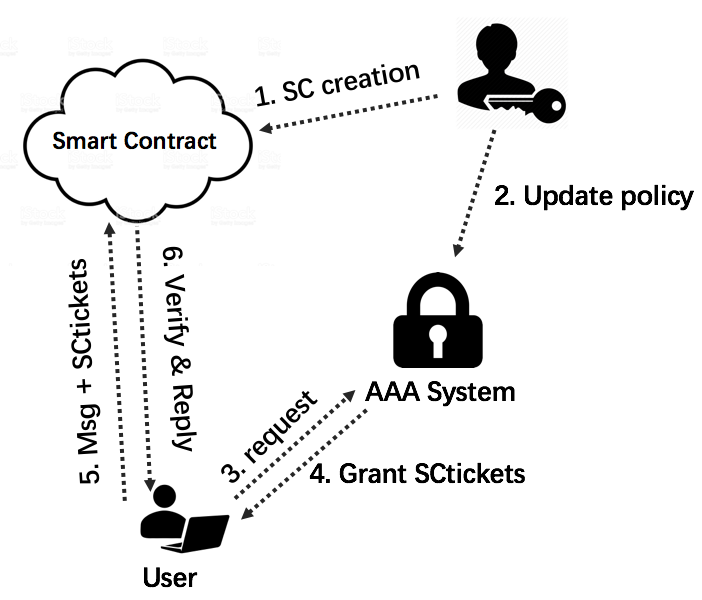
\includegraphics[width=0.7\linewidth]{fig/overview}
  \caption{A high-level overview of the SCtickets.}
  \label{fig:overview}
\end{figure}
\\\indent The central point of our design is a AAA platform that implements main functionalities: the SCtickets-related services and access policies management. The SCtickets-related services grant Users to SCtickets generated by the calling message of User and provide Owner with verification functionality corresponding to the SCtickets, while the latter functionality is used mainly for managing general access policies (e.g., insert, remove, update). Meanwhile, AAA is responsible for keeping public key and private key pair in local storage. The above-mentioned key pair is used for tickets signature and verification prcess and generated through web3.js by leveraging secp256k1 elliptic curve, aiming not to leaking the privacy of Owner account in Ethereum.
Assume that the Owner do have a valid location(address) of its smart contract in Ethereum network, every calling though different smart contracts is able to trigger a new transaction regardless of its gaslimit, gasprice.\\\indent 1 - In the first step, Owner synchronized its own policy to AAA when a new smart contract created by itself. Besides, Owner also generates new verification key-pair which is sent to AAA. AAA stores general policies corresponding to Owner’s rule as well as key pair.
\\ \indent 2 - User requests the SCtickets-generate service by sending transaction information that contains transaction message information before access to the Owner, such as msg.sender represents calling address and msg.sig represents calling specific function in Owner’s code, respectively.
\\\indent3 - The AAA notices the request and trigger SCtickets-generate service itself. First of all, AAA analyzes the parameters sent by User and determines access permission according to the policies matching. Then, if User have permission to Owner, AAA is able to generate a signature according to the SCtickets type using elliptic curve signature algorithm in Ethereum, where signer is Owner associated with its verification private key while message-to-be-signed suffix with current timestamp are based on diffrent SCtickets types accordingly. Finally, AAA transfers SCtickets to User. Tickets can be treated as a permission for Owner, like a visa for entry countries. However, if User fails to pass all the compulsory policies, AAA have right to refuse User’s access.
\\\indent4 - User send request to Owner after it hold a SCtickets. Once noticed the request, Owner firstly should verify the validation of SCtickets so as to be aware of tickets type, which smart contract is calling and executing its own code, which function can be called and the allowed calling time. Verification process is supposed to be done within Owner's code, parsing the signature to the public key corresponding to private key during signing process. Additionally, there are two types of function call, namely, external call and internal call. The former type raises a new transaction process from step 1 to step 4 repeatedly as every variable value of the SCtickets will be change in Solidity language and a new SCtickets will be granted for new User accordingly. On the other hand, the latter type just read/write internal methods without passing any SCtickets.
\\\indent5 - Every access period need to abide by blockchain timestamp in Ethereum network, leveraging UNIX global timestamp.  User can access to Owner by the expiry timestamp and, also, is able to apply for a new SCtickets in case of passing the requirements.
\\\indent6 - AAA, a strong proxy for authorizing permission and validating access, should not be a smart contract so as to every smart contract mined in blockchain is permanent and forever state and disallowed to changed while policies within AAA updates dynamically.
\\\indent7 - Owner maintains the right to refuse any calls if happens to unmatched verification despite User has been obtained valid SCtickets for the fact that malicious attack and fake signature issue.

\section{Architechture Details}
\label{sec:details}
\subsection*{4.1 SCtickets type}
- introduce details of tickets
\noindent The SCtickets types in AAA are presented in \autoref{fig:type}.
\begin{figure}[h!]
  \centering
  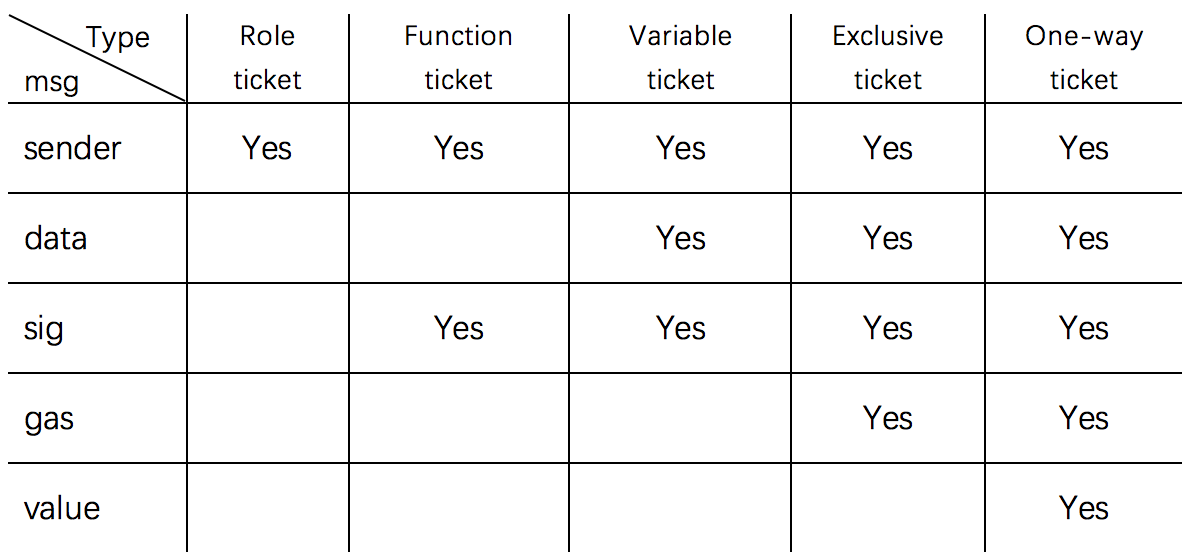
\includegraphics[width=1.0\linewidth]{fig/type}
  \caption{Different SCtickets types granted by AAA.}
  \label{fig:type}
\end{figure}
\\\indent Currently, AAA provides user with five different types of tickets, namely, role tickets, Tx tickets, function \& variable tickets, exclusive tickets and single permit. Different types of tickets should generate different signature which is to be verified by Owner accroding to different neccessary msg information.
\\\textbf{Role ticket}: is the highest priority tickets granted by AAA, meaning that certain caller(a.k.a User) could access to the smart contract before the expiry timestamp freely, regardless of functions, variables, times of sending transactions.
\\\textbf{Function ticket}: provides User with multiple transaction-sending access and full parameters. Hence, it is neccessary for AAA to get the information of msg.sender and msg.sig so as to Owner is aware of which method is to be called in every period of transaction.
\\\textbf{Variable ticket}: limits User to execute specific function code, and besides, variables. AAA parses first four bytes of the full msg.data and following bytes, which represent the function name and input parameters, respectively. Function \& variable ticket can protect some private data member in smart contract from being modified.
\\\textbf{Exclusive ticket}: disallowed other user to access smart contract which is called by current user. By default, other types of tickets are not exclusive by User. Assume that user, who is holding exclusive ticket, is calling the "setter" function of one smart contract. Exclusive ticket gurantees only one user is able to call certain smart contract. Other User will receive deny message from smart contract saying "the tickets is belong to other user now". However, it is not proper that only one user can access to certain contract as time period is too long, e.g., 1 week or 1 month, sometimes. Hence, Exclusive ticket need msg.gas for the fact that blockchain can notice the timestamp when obtaining msg.gas, which means remaining gas and transaction is done. After that, other User is able to access to previous smart contract.
\\\textbf{One-way ticket}: gurantees the User only get access to the smart contract one time though holding a valid SCtickets authorized by AAA system as the name implies. In order to generate one-trip ticket, AAA need to get as much as information to tag transaction well. When double-sending happends, smart contract emits deny User's access infomation if former transaction information has been stored.

\subsection*{4.2 Tickets implementation}
- introduce implementation tickets type 
- introduce each tickets msg data, usage, applicable scenario

\noindent \textbf{1a}): Owner represents the address that a smart contract is initially created. In Ethereum world, every valid account hold its own private key which could be regarded as an unique idendity. Obviously, the owner of a smart contract need to generate a key-pair only for signature and verification when constructing new smart contract and synchronize private key with AAA party. Firstly, Owner uses keccak256(private\_key, nounce) to produce a new private key where private\_key represents its own account pk and nounce only valid for current smart contract. After that, a new key-pair is created by getting the return value of privateKeyToAccount(). We define a localStorage object, namely, keyStorage, to store address-to-privatekey mapping in AAA and this object is essential to Node.js storage package. Meanwhile, keep the public key of above-mentioned key-pair in Owner's smart contract for verified signature.
\\\noindent \textbf{1b}): Policies vary in different smart contracts and could be customized by Owner. Compared with key-related API, Owner is also supposed to update its own policies with AAA. Like key pair, AAA maintains a policy storage area to save all the policies corresponding to certain Owner. Currently,  every single policy struct has two member for test convenience: balance, to rule the access balance limit; time, to set access period. Like 1a), AAA also provides APIs which Owner is able to add, delete, update policies. 
\\\noindent \textbf{2a,2b,2c}): Once completely updated policy and synchronized private key to AAA, Owner is to be called by User all the time. This process starts with applyTickets(type, msg, policy\_info) defined in AAA system. First of all, User calls applyTickets() function with the input argument of type, namely, tickets type, msg, calling data and policy\_info, which contains ample value of User. And then, AAA is responsible for determining if User meets policies defined by Owner by matching every rules in policy structure. If lucky, AAA grants valid ticket to User. A valid ticket contains several data parts: one is tickets type. At present, we tag five types of tickets discussed in Chapter4.1 from integer 1 to 5 representing five types respectively. Signature part contains signed data by Owner private key generated by web3.eth.accounts.sign() in web3.js package and hash of msg for following signature validation process. The value of msg varies according to diffrent tickets type. More importantly, ticket definitely returns timestamp value to Owner so as to synchronize the access peroid between Owner and User.
\\\noindent \textbf{3a}): User sends transaction to the smart contract of Owner after obtaining valid tickets from AAA. In our case, setA() function, defined in Owner smart contract, is to alter value of a, which is an uint type storage in Owner. We assume that User is willing to update a's value by calling Owner.setA() along with ticket dicussed above.
\\\noindent \textbf{3b}): After noticing the calling message from User, Owner implement verified() to gives priority to verify the validation of ticket. Normally, the validation process need to be done two steps. One is vefify the current timestamp \textgreater  access period or not. Second step is done by wrapping parseTickets() function which accepts two parameter, hash of message and signature. Owner needs to parse the signature manually and retrieve three parameters r, s, and v, the first 32 bytes of signature, the 33-64 bytes of signature and the recover arguments for ECC respectively. In ethereum, the value of v is usually set 27. Finally, we get the public key which is corrensponding to the private key signing the message by leverage the ecrecover() in Solidity. If the return valus equals to the address of Owner, which means the ticket verified successfully, User can hold this valid tickets to access to the Owner's smart contract. Furthermore, there needs to be one more step for one-trip ticket. Owner need to look for and determine if the id is in set or not.


\subsection*{4.3 One-way tickets}
- introduce motivation, backgroud, difficulty, scenario
- introduce implementation, bit-map synchronization process

\subsection*{4.4 Tickets among Multiple smart contract}
- introduce tickets transfer among external calling contract
- introduce append tickets and updated tickets verification process





\section{Policy}
\label{sec:policy}
- introduce policy concept
\subsection*{5.1 blacklist and whitelist}

\subsection*{5.2 Hydra user case}
- integrity Hydra to test illegal sender

\subsection*{5.3 involvement}
- make the rule related account balance 





\section{Security discuss}
\label{sec:security}
\subsection*{6.1 private-key preserve}
- verification key pair

\subsection*{6.2 tickets-forge attack}
- signature

\subsection*{6.3 timestamp}





\section{Realization in Practice}
\label{sec:implementation}
\subsection*{7.1 Overview}
- introduce implementation environment
- introduce assumption
\noindent To implement a prototype of the proposed framework, we used the Ethereum smart contract and Ganache Testnet implementation. We created the smart contracts by Solidity and configured Ganache as an Ethereum network environmnet. It ran under Solidity compiler version 0.4.24 with Ganache 1.1.0. We also leveraged Truffle, a popular framework in Ethereum with the version v4.1.14, and web3.js 1.0.0-beta.35, a collection of modules which contain specific functionality for the ethereum ecosystem. Currently, the AAA provides service as an JavaScript file, which is run under Node.js v10.2.1 bundled with node-localStorage package for storing general policies and verification key-pairs.

Specific AAA implementation is presented in \autoref{fig:imple}.
\begin{figure}[h!]
  \centering
  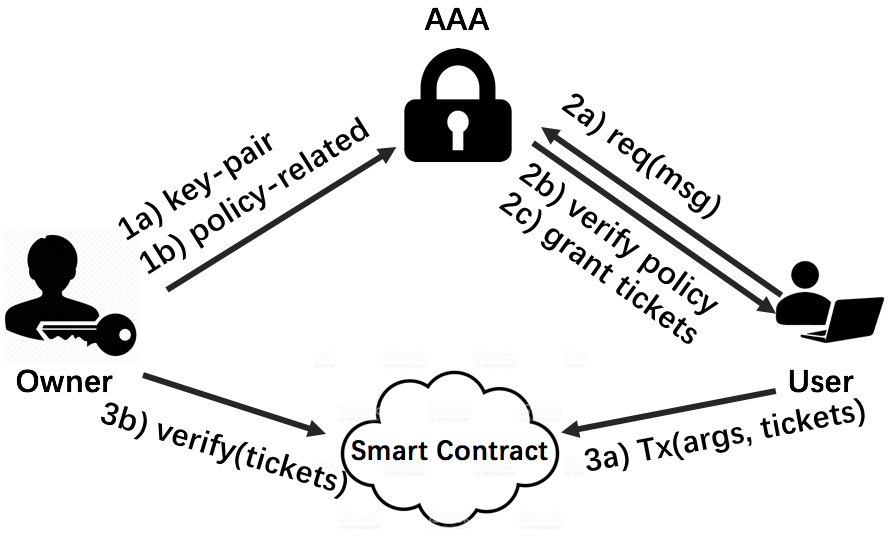
\includegraphics[width=1.0\linewidth]{fig/imple}
  \caption{Specific AAA implementation.}
  \label{fig:imple}
\end{figure}

\subsection*{7.2 Details}
- introduce each entities 

\subsection*{7.3 Evaluation}
- introduce overhead
- storage cost
- gas cost
- build model(if applicable)




% \section{Analysis}
% \label{sec:analysis}
% Analysis
- Overhead (computation and communication)
- Practicality
- Security analysis
Evaluation
- Compare with related work!
- Deployment issues (legacy issues?)



\section{Related work}
\label{sec:related}
Related work
- Analyze research landscape, how does the work fit in?
- Present work that others may think to be related and explain why it
  isn't related

\cite{1176982}


\section{Conclusions}
\label{sec:conclusions}
Conclusion
- What have you learnt from the research? What are surprising findings
  from the work? What future work is possible? Some additional
  insights. The conclusion is very different from the abstract!


--------------------------------------------------------------------------------
Imagine a drunken reviewer who reads the paper, will s/he understand?
Is the paper sufficiently clear that even a drunken reviewer gets it?
--------------------------------------------------------------------------------
- Replace an assumption by an observation. It's much easier to disagree
  with an assumption than with an observation!
- Always keep the reader informed on where in the paper s/he is, where
  the paper is heading toward, always make it clear what else is
  expected, what is still coming up
- Make sure that mechanism is concisely explained, so that results are
  repeatable.
- State the main result upfront, then back it up with the text. Poor
  writing is to explain things in a lot of text and the main point
  doesn't really jump out. For example, in poorly structured text the
  reader has to pay careful attention to assemble the train of thought
  as she's reading the section.
- Use phrases such as "we find that", "we discovered that"
- Use "because" often, people seem to believe whatever comes thereafter.
- Careful with the terms "correct", "optimal", or "proof"! People have
  varying opinions of correctness, so it's likely that someone
  misunderstands it. Especially theory people are very particular
  about this term.



\section*{Acknowledgment}
\label{sec:ack}
\lstset{language=python}
\begin{lstlisting}
n, p = 1000, 1/6.0
s = np.random.binomial(n, p, 1000)
plt.figure()
plt.hist(s, color='red', density=True, bins='auto')

def factorial(x):  
    int_x= int(round(x))
    fact=1
    for i in range(int_x+1)[1:]:
        fact=fact*i
    return fact

def probabilityFunc(x):
    mean = 3.25;
    return np.power(mean, x) * 1.0 / np.exp(mean) / np.math.factorial(x);

print probabilityFunc(0)+probabilityFunc(1)+probabilityFunc(2)

#for the mean is known
def calUncert(n, p):
    var = n * p * (1-p);
    return var;

def standardVar(n, p):
    variance = calUncert(n, p);
    return np.sqrt(variance);


n_sample = 752 + 283
p_sample = 752.0 / n_sample
def calstandVarWed(n, p):
    return standardVar(n, p);

print calstandVarWed(n_sample, p_sample)


def cal():
    mean = 0.75 * (752 + 283);
    variance = np.sqrt(0.75 * (752 + 283) * 0.25);
    return 2 * ss.norm(mean, variance).cdf(752);
    

print cal()

\end{lstlisting}


\bibliographystyle{plain}
\bibliography{ref}
\end{document}

%%% Local Variables: 
%%% mode: latex
%%% TeX-master: t
%%% End: 
